\begin{figure}[htbp]
\centering
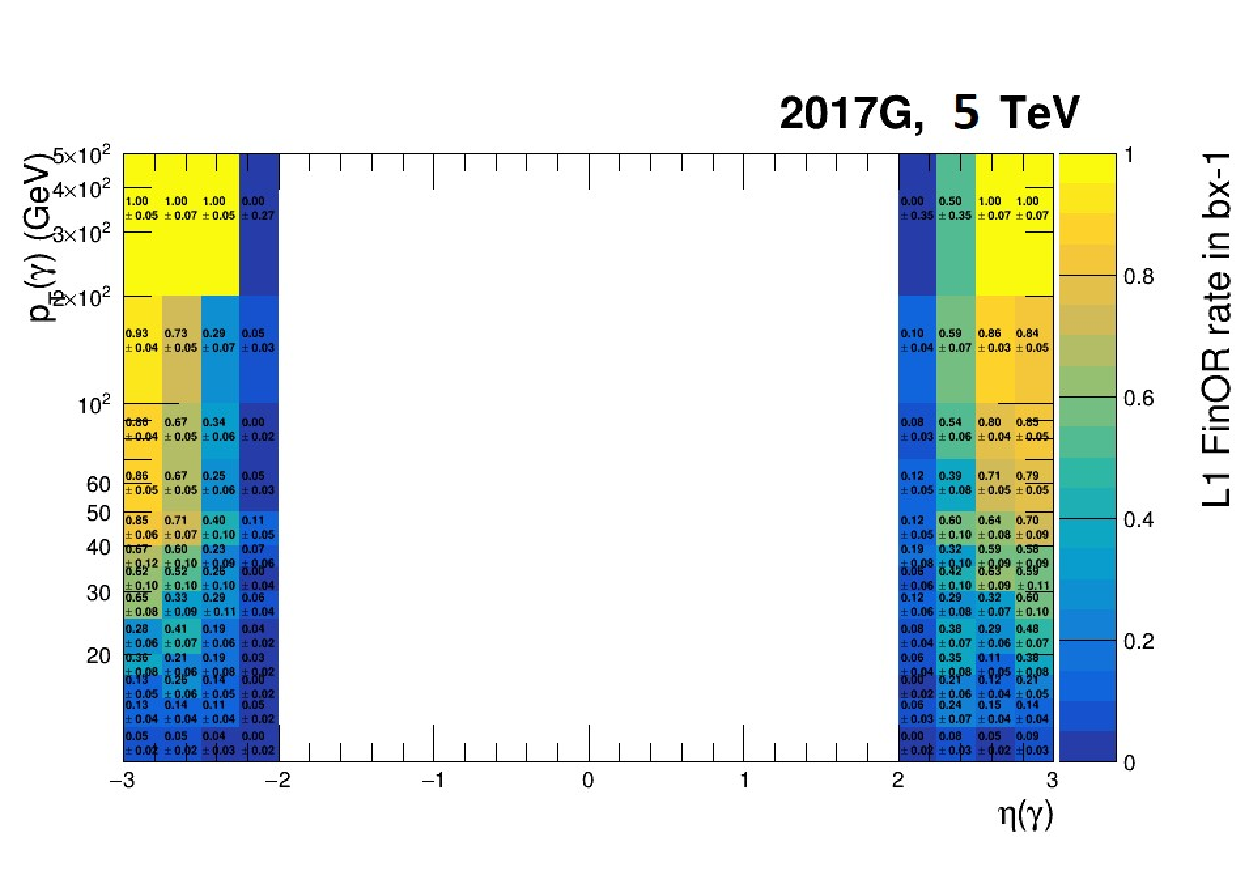
\includegraphics[width=0.49\textwidth]{plots/Prefire/L1prefiring_photonpt_2017G.pdf}
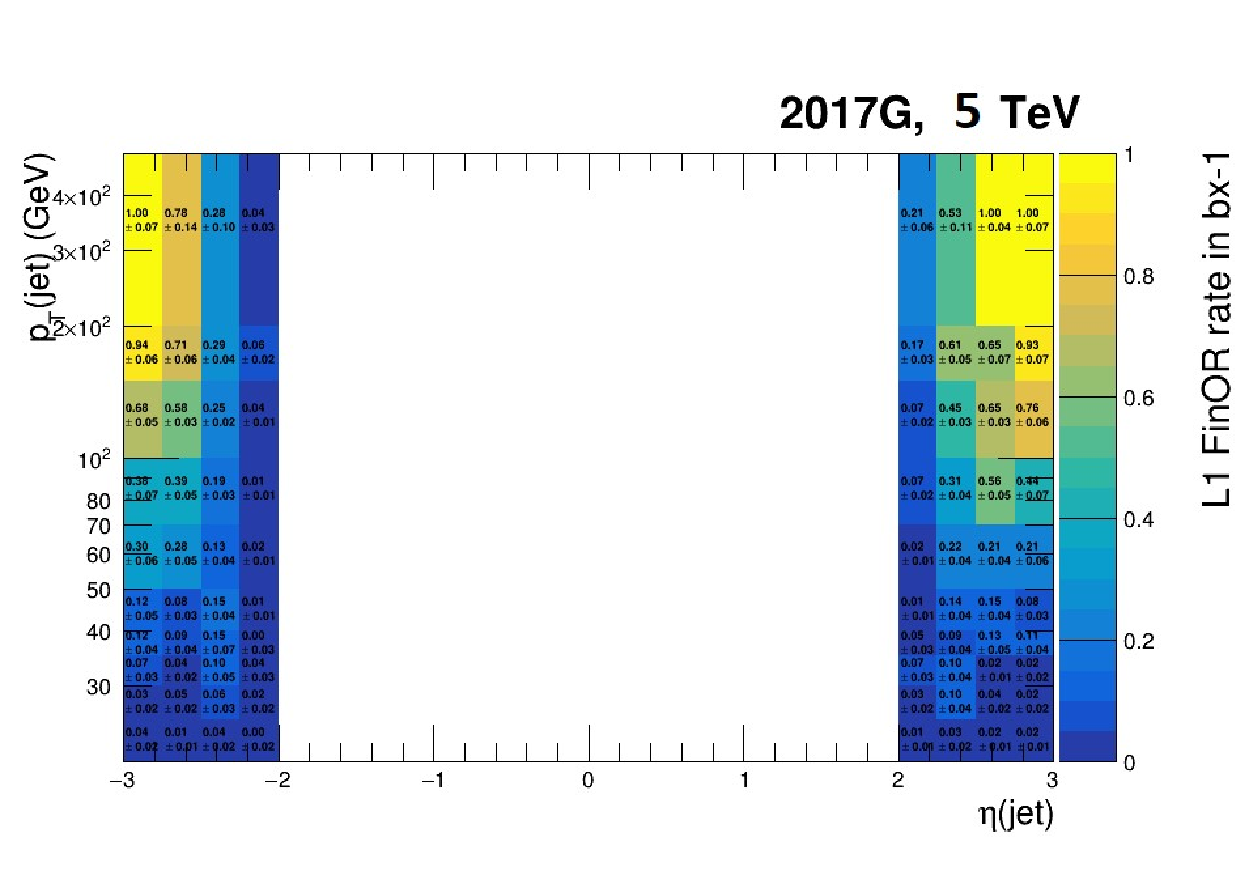
\includegraphics[width=0.49\textwidth]{plots/Prefire/L1prefiring_jetpt_2017G.pdf}
\caption{Pre-firing probability maps for photons (left) and jets (right) for 2017G (\sg). The $z-\mathrm{axis}$ represents the probability of an object with $(\pt,\eta)$ causing pre-firing. Objects with higher \pt and $|\eta| \sim 3$ are more likely to cause pre-firing. Objects with $|\eta| < 2$ do not cause pre-firing.}
\label{fig:prefire:2017G}
\end{figure}

\begin{figure}[htbp]
\centering
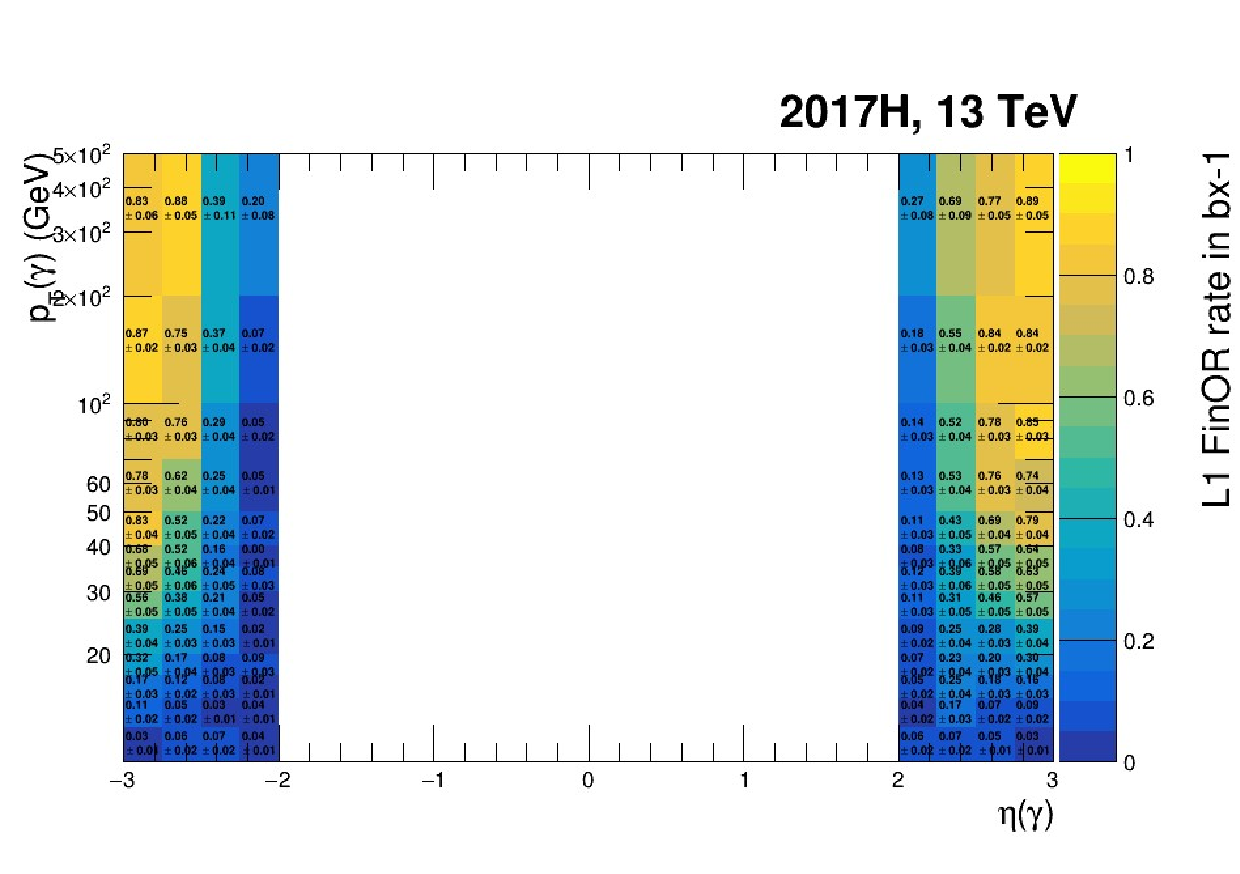
\includegraphics[width=0.49\textwidth]{plots/Prefire/L1prefiring_photonpt_2017H.pdf}
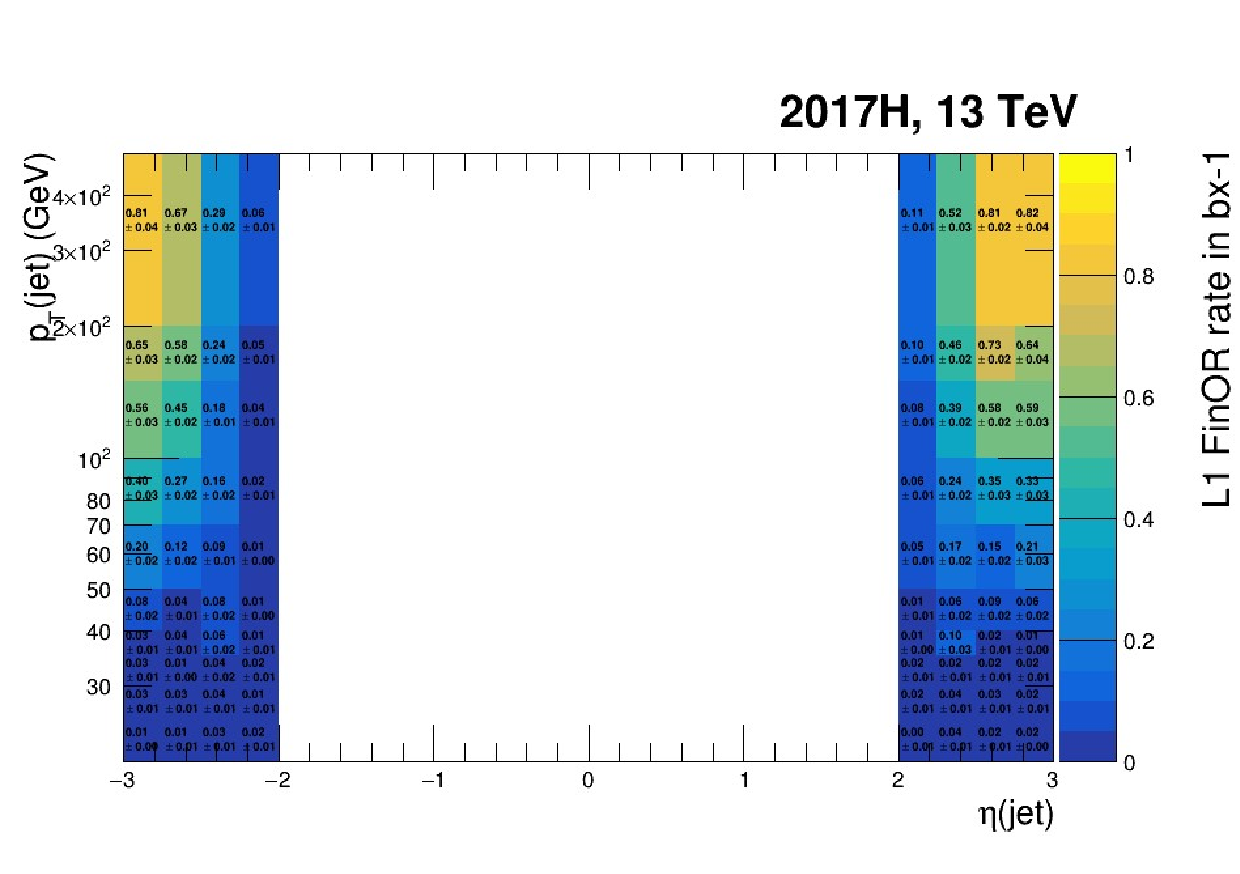
\includegraphics[width=0.49\textwidth]{plots/Prefire/L1prefiring_jetpt_2017H.pdf}
\caption{Pre-firing probability maps for photons (left) and jets (right) for 2017H (\sh). The $z-\mathrm{axis}$ represents the probability of an object with $(\pt,\eta)$ causing pre-firing. Objects with higher \pt and $|\eta| \sim 3$ are more likely to cause pre-firing. Objects with $|\eta| < 2$ do not cause pre-firing.}
\label{fig:prefire:2017H}
\end{figure}